\chapter{TINJAUAN PUSTAKA}

\section{PT Bisma Jaya}

PT Bisma Jaya merupakan perusahaan yang bergerak di industri transportasi angkutan laut yang berbasis di Balikpapan, Kalimantan Timur. Sejak tahun 2011, perusahaan telah menyediakan berbagai jenis kapal untuk kebutuhan transportasi industri. Dalam menjalankan tugasnya PT Bisma Jaya memiliki struktur organisasi seperti pada Gambar 2.1.

\begin{figure}[!h]
    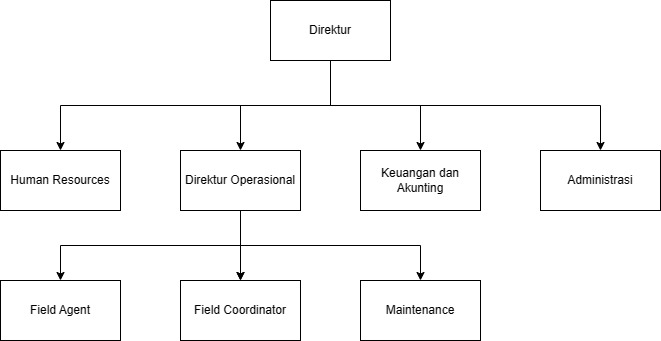
\includegraphics[width=1\linewidth, center]{images/tinjauan-pustaka/fig-org-structure.jpg}
    \caption{Struktur Organisasi PT Bisma Jaya}
    \label{fig:org-structure}
\end{figure}

Gambar 2.1 memberikan gambaran struktur organisasi dari PT Bisma Jaya yang dipimpin oleh Direktur yang membawahi \textit{Human Resource}, Direktur Operasional, Keuangan dan Akunting, dan Administrasi. Direktur Operasional membawahi beberapa bagian seperti \textit{Field Agent}, \textit{Field Coordinator}, dan \textit{Maintenance}. Seluruh kegiatan operasional kapal berada dalam tanggung jawab Direktur Operasional yang memastikan seluruh operasi berjalan dengan lancar serta membuat keputusan strategis dalam mengelola biaya operasional.

Dalam penelitian ini, peneliti akan lebih banyak berkomunikasi dengan Direktur Operasional. Diharapkan Sistem Monitoring yang akan dibuat dapat memberikan wawasan mengenai performa armada kapal sekaligus menjadi acuan dalam keputusan jadwal pengisian bahan bakar.


\section{\textit{Internet of Things}}

\textit{Internet of Things (IoT)} merujuk pada keterhubungan antara obyek, perangkat, mesin satu dengan lainnya dan internet mengizinkan mereka untuk mengumpulkan dan menukar data \parencite{inproc:gazis}. Secara arsitektur IoT dapat dibagi menjadi 4 lapisan utama: \textit{sensing layer}, \textit{network layer}, \textit{data processing layer}, dan \textit{application layer} \parencite{article:sikder}. Detailnya dapat dilihat pada Gambar 2.2

\begin{figure}[ht]
    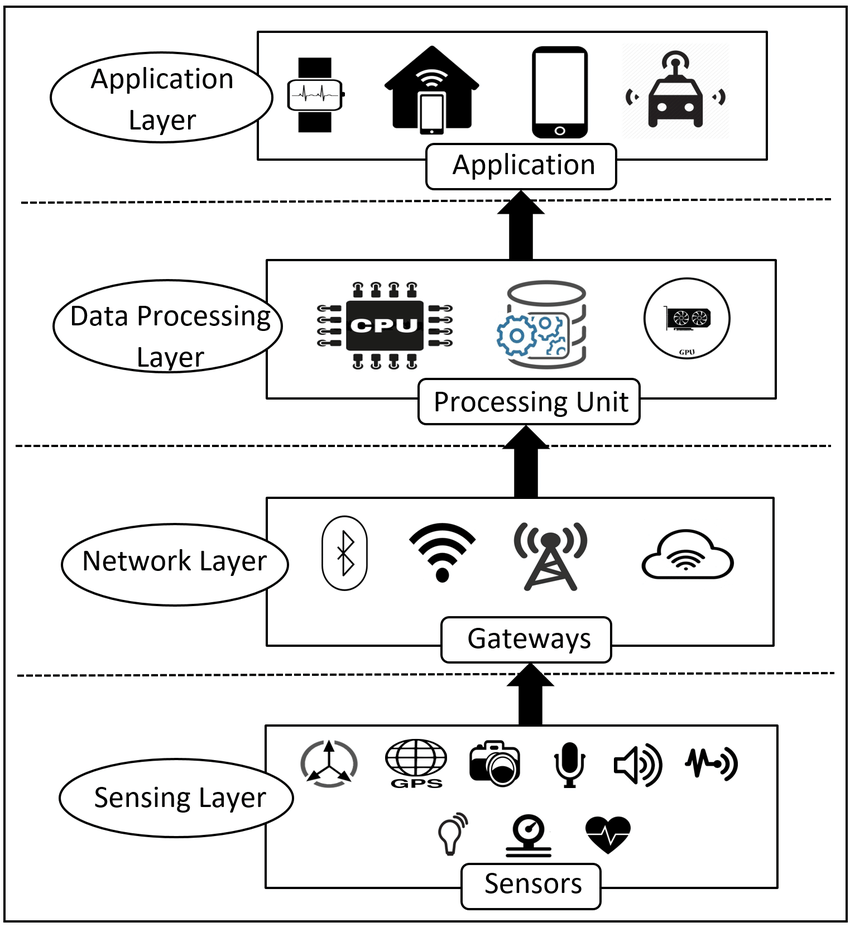
\includegraphics[width=0.6\linewidth, center]{images/tinjauan-pustaka/fig-iot-architecture.png}
    \caption{Lapisan dan Komponen Arsitektur IoT \parencite{article:sikder}}
    \label{fig:iot-architecture}
\end{figure}

Berikut gambaran umum pada setiap lapisan:
\begin{enumerate}
    \item \textbf{\textit{Sensing Layer}}

    Lapisan ini bertanggung jawab untuk memanfaatkan berbagai sensor dan perangkat untuk mengumpulkan data. Sensor seringkali memberikan data berupa angka mentah seperti tegangan. Oleh karena itu, perangkat IoT dapat memprosesnya terlebih dahulu sebelum dikirim ke server - disebut juga dengan \textit{edge-computing} - atau langsung meneruskan data tersebut ke lapisan jaringan untuk diproses di server.


    \item \textbf{\textit{Network Layer}}

    Lapisan ini bertugas mengirimkan data yang diperoleh sensor ke lapisan pemrosesan data untuk diolah. Lapisan ini juga bertugas mengawasi bagaimana perangkat jaringan IoT berkomunikasi satu sama lain. Untuk menjaga keamanan komunikasi, digunakan token autentikasi setiap adanya pengiriman data ke \textit{server}.

    \item \textbf{\textit{Data Processing Layer}}

    Pemrosesan dan analisis data sensor berada di bawah lingkup lapisan ini. Selain itu, ia bertugas mengelola dan menyimpan data. Lapisan pemrosesan data sangat penting untuk menghasilkan wawasan berharga dan mengambil tindakan yang sesuai berdasarkan data yang dikumpulkan.

    \item \textbf{\textit{Application Layer}}

    Dengan menggunakan data yang dikumpulkan dan diproses, lapisan ini bertanggung jawab untuk memberikan \textit{actionable insight} kepada pengguna akhir. Lapisan ini juga bertugas memastikan kerahasiaan dan keamanan data yang diproses dan dianalisis dan merupakan lapisan teratas dalam arsitektur IoT.

\end{enumerate}

\section{Raspberry Pi}
Raspberry Pi merupakan \textit{single-board computer} (SBC) yang telah mendapatkan perhatian dan popularitas yang signifikan dalam beberapa tahun terakhir. Teknologi inovatif ini memungkinkan berbagai penerapan dan sekarang penting dalam bidang ilmu dan teknik komputer \parencite{article:johnston}. Raspberry Pi adalah pilihan yang bagus untuk aplikasi \textit{Internet of Things} (IoT) karena portabilitasnya, paralelismenya, keterjangkauannya, dan konsumsi dayanya yang rendah \parencite{article:hosny}. Hal yang membuat Raspberry Pi dapat diandalkan sebagai perangkat IoT adalah adanya 40 pin GPIO yang memungkinkan ia dihubungkan ke beragam sensor dengan berbagai \textit{interface}. Raspberry Pi serta informasi GPIO dapat dilihat pada Gambar 2.3.

\begin{figure}[!h]
    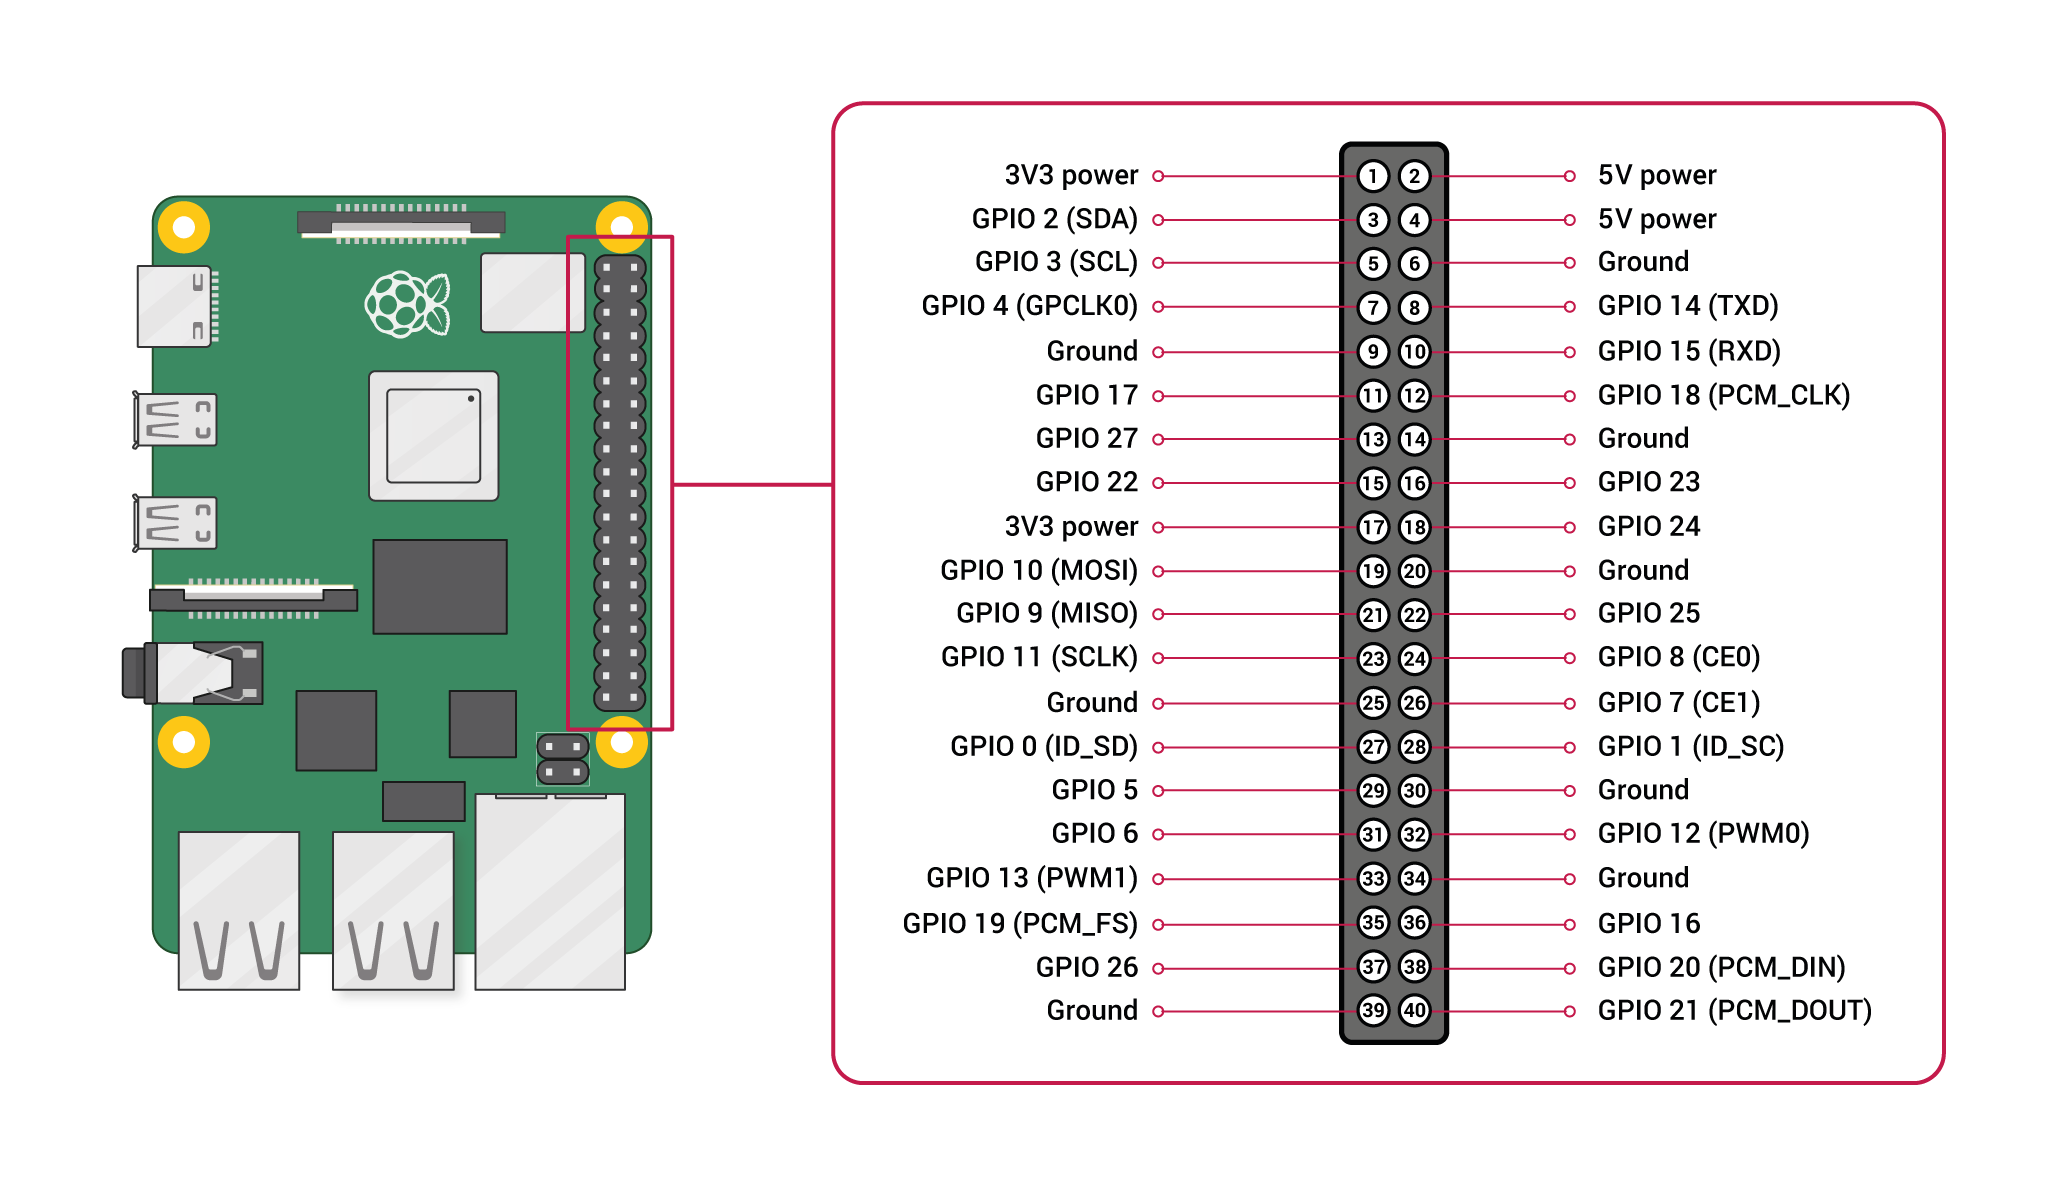
\includegraphics[width=1\linewidth, center]{images/tinjauan-pustaka/fig-raspy.png}
    \caption{Raspberry Pi dan 40 pin GPIO}
    \label{fig:raspy}
\end{figure}

Setiap pin GPIO dapat digunakan sebagai pin input maupun output, dan dapat digunakan untuk berbagai kebutuhan. Terdapat pin 5v dan 3.3v yang berjumlah masing-masing 2, juga beberapa pin \textit{ground} yang tidak dapat dikonfigurasi. Sisanya merupakan pin \textit{general purpose} 3.3v, yang berarti  output diatur ke 3.3v dan input toleran dengan nilai 3.3v. Pin output dapat diatur ke \textit{high} (3.3v) dan \textit{low} (0v). Begitu juga dengan pin input, dapat membaca \textit{high} (3.3v) dan \textit{low} (0v). Selain itu, pin GPIO juga dapat digunakan untuk kebutuhan yang memerlukan jenis pin yang spesifik seperti \textit{PWM (pulse-width modulation)} untuk membuat sinyal analog; \textit{SPI (serial peripheral interface)} untuk transfer data antar Raspberry Pi dengan perangkat periferal; \textit{I2C (inter-integrated circuit)} untuk komunikasi dengan berbagai jenis sensor; dan Serial untuk pembacaan data serial.

\section{Perbandingan SDLC}

Berikut adalah perbandingan dari metodologi \textit{Extreme Programming} dengan salah satu metode \textit{sequential}, yaitu Waterfall dan metode Agile lainnya, yaitu Scrum menurut \textcite{inproc:fahrurrozi} dan \textcite{article:suryantara}.

\newpage

\begin{longtable}[!h]
        {
            p{0.19\textwidth}
            p{0.27\textwidth}
            p{0.27\textwidth}
            p{0.27\textwidth}
        }
        \caption{Perbandingan metodologi SDLC} \\

        \hline
            Tahapan dalam pengembangan &
            \textit{Extreme Programming} &
            \textit{Waterfall} &
            Scrum \\ [0.5ex]
        \hline

        \endfirsthead

        % \multicolumn{3}{@{}l}{\ldots continued} \\

        \hline
            Tahapan dalam pengembangan &
            \textit{Extreme Programming} &
            Waterfall &
            Scrum \\ [0.5ex]
        \hline
        \endhead % all the lines above this will be repeated on every page
        \hline

        % \multicolumn{3}{r@{}}{continued \ldots} \\
        \endfoot
        \hline
        \endlastfoot

        \textit{Planning}
        &
        Pada tahap ini dilakukan pengumpulan kebutuhan sistem dan menjadikannya dalam bentuk \textit{user story} dan diurutkan berdasarkan tingkat kesulitannya. Developer kemudian memutuskan \textit{user story} apa saja yang akan dikerjakan pada iterasi mendatang.
        &
        Tahap ini merupakan langkah awal dimana kebutuhan proyek dikumpulkan dan dianalisis.
        &
        Tahap ini dibagi menjadi 2 bagian: Sprint Planning dan Release Planning. Sprint Planning dilakukan setiap awal sprint dan melibatkan tim untuk memilih pekerjaan yang akan mereka selesaikan di sprint tersebut. Release Planning dilakukan setiap awal rilis dan melibatkan tim merencanakan fitur yang akan dimasukkan ke rilis tersebut.

        \\
        \midrule

        \textit{Analysis}
        &
        \textit{User story} kemudian dianalisis dan dibuat menjadi task yang dapat dikerjakan.
        &
        Pada Tahap ini kebutuhan yang dikumpulkan akan dipecahkan menjadi potongan yang dapat dikelola.

        &
        Analisis terjadi saat Sprint \textit{Planning}, dimana tim akan memilih perkerjaan yang akan mereka selesaikan di sprint tersebut

        \\
        \midrule

        \textit{Design}
        &
        Tim bekerja dalam iterasi singkat untuk menghasilkan software yang berfungsi, dan desainnya berkembang seiring kemajuan proyek.
        &
        Tahap desain melibatkan pembuatan rencana rinci untuk software berdasarkan persyaratan yang dikumpulkan dalam fase perencanaan dan analisis.
        &
        Perancangan terjadi selama Sprint \textit{Planning}, dimana tim memilih pekerjaan yang akan mereka selesaikan selama sprint.

        \\
        \midrule

        \textit{Implementation}
        &
        Pengembang bekerja dalam waktu singkat untuk menghasilkan software yang berfungsi, dan implementasinya berkembang seiring kemajuan proyek.
        &
        Tahap implementasi melibatkan koding software berdasarkan rencana rinci yang dibuat pada fase desain.
        &
        Implementasi terjadi selama sprint, dimana tim menyelesaikan pekerjaan yang mereka pilih selama Sprint \textit{Planning}.

        \\
        \midrule

        \textit{Support \& Security}
        &
        Support dan security adalah proses yang berlangsung sepanjang proyek. Tim bekerja dalam waktu singkat untuk menghasilkan software yang berfungsi, dan perangkat lunak tersebut terus diperbarui dan dipelihara.
        &
        Tahap support dan security terjadi setelah software dikirimkan. Tahap ini melibatkan pemeliharaan dan pembaruan perangkat lunak untuk memastikannya terus memenuhi kebutuhan pengguna.
        &
        Support dan security terjadi setelah perangkat lunak dikirimkan. Fase ini melibatkan pemeliharaan dan pembaruan perangkat lunak untuk memastikannya terus memenuhi kebutuhan pengguna.
        \\ [1ex]

    \label{tab:sdlc-comparison}
\end{longtable}

Secara garis besar, \textit{Software Development Life Cycle} memiliki lima tahapan, yaitu \textit{Systems Planning}, \textit{Systems Analysis}, \textit{Systems Design}, \textit{Systems Implementation}, dan \textit{System Support and Security}. Metode \textit{Sequential} dan \textit{Agile} memiliki cara implementasi yang cukup berbeda. Pada metode sekuensial seperti Waterfall, perangkat lunak dikembangkan secara linear. Artinya, sebelum tahap selanjutnya, tahap sebelumnya sudah harus diselesaikan. Adanya perbedaan atau perubahan mengharuskan pengembang untuk kembali ke tahap awal. Sedangkan, pada metode \textit{Agile} seperti \textit{Extreme Programming (XP)} atau Scrum, aktivitas di tahapan-tahapan tersebut dapat secara dinamis berubah dan akan menyesuaikan kembali di tahapan sebelumnya. Oleh karenanya, metode sekuensial tidak akan dipilih pada penelitian ini.

Lebih lanjut, komparasi antara metode \textit{Agile} yaitu XP dengan Scrum pada fase perencanaan. Pada XP, perencanaan dilakukan menjadi dua bagian, yakni \textit{Release Planning} dan \textit{Iteration Planning}. Tujuan \textit{Release Planning} adalah untuk mengetahui fitur apa saja yang diperlukan sistem dan kapan fitur tersebut dikerjakan. Lalu, terdapat \textit{Iteration Planning} yang dilakukan setiap awal iterasi. Pada fase ini, pengembang menyiapkan rencana untuk mengimplementasi fitur yang pada rilis saat itu. Kemudian kebutuhan sistem akan dibuat menjadi task berdasarkan \textit{user story} yang dibuat. Urutan pengerjaan akan dikelompokkan menjadi Iterasi yang berisi kumpulan \textit{user story} yang telah diprioritaskan. Pengerjaan teknis yang dilakukan selama iterasi meliputi analisis, desain sederhana, pengkodean, dan testing. Sedangkan untuk Scrum, perencanaan dibagi menjadi dua bagian yakni \textit{Sprint Planning} dan \textit{Release Planning}. Singkatnya, \textit{Release Planning} berisi seluruh fitur yang akan dikembangkan dan pengerjaannya dibuat menjadi backlog yang kemudian akan dibagi di \textit{Sprint Planning} di setiap awal sprint.

Pada tahap implementasi, XP dan Scrum sebenarnya tidak begitu jauh berbeda karena mengadopsi pendekatan yang sama. Namun, terdapat beberapa perbedaan utama diantara keduanya. Pertama, satu iterasi (yang disebut dengan sprint) pada Scrum dikerjakan selama 2 pekan hingga 1 bulan. XP mengerjakan satu iterasi lebih singkat yakni hanya 1 hingga 2 pekan saja; Kedua, sprint tidak boleh diubah selesai ditetapkan ketika \textit{sprint planning}. Komitmen harus dipegang untuk menyelesaikan item backlog. XP lebih fleksibel terhadap perubahan dalam iterasi selama fitur tersebut belum dikerjakan. Task dengan ukuran sebanding dapat ditukar ke iterasi sebagai ganti dari fitur yang belum dimulai; Ketiga, pengerjaan fitur pada XP ditentukan oleh urutan prioritas. Sedangkan pada Scrum, prioritas backlog tidak menjadi acuan dalam penentuan item yang akan dikerjakan di suatu Sprint, karena bisa jadi pengembang yang akan mengerjakan fitur tersebut harus fokus dengan item yang memiliki prioritas yang tinggi pada sprint yang sama. 

Pada akhirnya, dalam penelitian ini dipilihlah metode Exteme Programming (XP) dengan beberapa pertimbangan seperti perbaikan atau penambahan fitur baru ditengah fase iteration to release, juga dari hasil jurnal dengan judul serupa. Riset yang dilakukan Rumandan (2023), berfokus pada pengembangan sistem informasi \textit{
customer service} menggunakan metode \textit{Extreme Programming (XP)} dimana ia menggaris bawahi kemampuan XP dalam memungkinkan interaksi pengguna secara langsung sehingga dapat segera menangani informasi dan resolusi komplain. \textcite{article:matharu} mendeskripsikan XP sebagai metodologi yang mendukung pengembangan perangkat lunak secara iteratif oleh tim skala kecil, sehingga meningkatkan produktivitas dan kualitas perangkat lunak untuk memenuhi kebutuhan yang terus berkembang.

\section{\textit{Extreme Programming} (XP)}

\textit{Extreme Programming} (XP) adalah pendekatan \textit{agile software development} yang memberikan penekanan pada kerja sama, pengembangan iteratif dan berulang, serta kemampuan beradaptasi terhadap perubahan kebutuhan. XP merupakan metodologi sederhana yang dibuat untuk tim pengembang kecil yang bertujuan untuk meningkatkan kualitas dan produktivitas perangkat lunak \parencite{article:matharu}. Kesulitan yang ditimbulkan oleh siklus pengembangan yang panjang dalam praktik pengembangan perangkat lunak konvensional menyebabkan terciptanya XP \parencite{article:rao}.

Ada berbagai prinsip dasar yang mendefinisikan XP. \textit{Continuous planning}, yang memerlukan komunikasi dan kolaborasi rutin antara pengembang dan pemangku kepentingan untuk memastikan bahwa tujuan dan persyaratan proyek dipahami dan dipenuhi \parencite{article:matharu}. Siklus hidup pada metode \textit{Extreme Programming} meliputi \textit{Exploration Phase}, \textit{Planning Phase}, \textit{Iteration to Release Phase}, \textit{Productionizing Phase}, \textit{Maintenance Phase}, dan \textit{Death Phase}. Lebih lengkapnya dapat dilihat pada gambar berikut.

\begin{figure}[ht]
    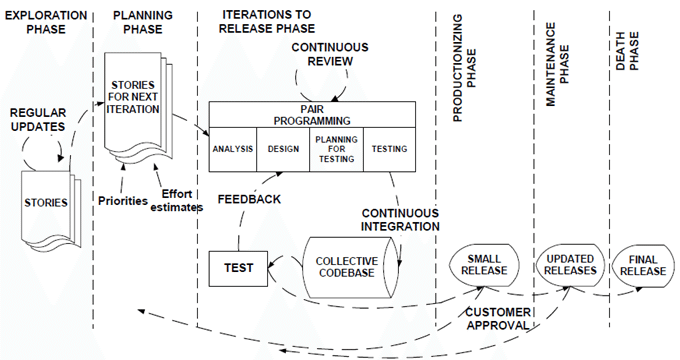
\includegraphics[width=1\linewidth, center]{images/tinjauan-pustaka/fig-xp-lifecycle.png}
    \caption{Siklus Hidup Metode \textit{Extreme Programming} \parencite{article:anwer}}
    \label{fig:xp-lifecycle}
\end{figure}

Berikut penjalasan detail untuk setiap fase:
\begin{enumerate}
    \item \textbf{Exploration Phase:}
    Pada fase ini, dihasilkan \textit{user story} yang dibuat berdasarkan hasil pengambilan data baik dari observasi, interview, dan dialog dengan mitra. \textit{User story} ini dapat bertambah seiring waktu mengikuti kebutuhan mitra.

    \item \textbf{Planning Phase:}
    Selanjutnya, \textit{user story} yang sebelumnya dibuat akan dikumpulkan dan diprioritaskan berdasarkan perhitungan poin story. Ini akan membantu kita dalam menentukan \textit{user story} mana yang akan dikerjakan pada iterasi berikutnya.

    \item \textbf{Iteration to Release Phase:}
    Tahap iterasi merupakan tahap dimana pengembang akan mengimplementasi sistem berdasarkan \textit{user story} yang ditentukan. Pertama, dilakukan tahap analisis untuk mengonversi kebutuhan mitra menjadi user flow untuk desain tampilan dan algoritma untuk logika sistem. Lalu, dilakukan desain tampilan sesuai dengan user flow yang dihasilkan dan dilakukan perencanaan untuk pengujian. Terakhir, dilakukan pengujian oleh pengembang sebelum kode diunggah ke repositori. Proses programming dilakukan secara parallel dari tahap analisis hingga pengujian. Setelah sistem berhasil melewati unit test dan integration test, sistem akan diuji oleh mitra dan hanya dapat lanjut ke tahap berikutnya setelah mendapatkan persetujuan.

    \item \textbf{Productionizing Phase:}
    Sistem yang telah diunggah di repositori akan diluncurkan di server dengan mode development. Ini memungkinkan mitra untuk melakukan pengujian fitur yang masih dalam proses persetujuan serta memberikan umpan balik secara berkala.

    \item \textbf{Maintenance Phase:}
    Iterasi yang mendapatkan persetujuan selanjutnya akan diluncurkan pada tahap ini. Dapat dikatakan sistem yang terdapat pada tahap ini merupakan gambaran terakhir dari sistem secara keseluruhan.

    \item \textbf{Death Phase:}
    Ini merupakan tahap terakhir dimana sistem akan diluncurkan secara penuh di server dengan mode production.
\end{enumerate}

Melihat dari tantangan industri mitra yang dinamis serta perlunya kolaborasi yang kuat dari berbagai lintas disiplin ilmu untuk mewujudkan Sistem Monitoring berbasis IoT ini, diputuskanlah metode Extreme Programming sebagai metodologi pengembangan perangkat lunak yang menekankan pada komunikasi dan kolaborasi serta sifatnya yang agile memungkinkan pengembang untuk menjawab berbagai tantangan industri tanpa interupsi selama proses pengembangan sistem.

\section{\textit{User Story}}

User story merupakan deskripsi singkat sebuah fitur dari perspektif pengguna akhir, biasanya ditulis dengan format seperti berikut 'As WHO, I want WHAT, so that WHY' (Dwitama dan Rusli, 2020).  Menurut Raharjana dkk. (2023) User story merupakan bagian fundamental dari pengembangan agile dengan membantu pengembang dalam memahami kebutuhan pengguna dengan efektif. User story sendiri tidak hanya digunakan untuk melakukan pengumpulan kebutuhan tetapi juga dapat dikonversi menjadi automated test case sehingga mempercepat proses testing.

Pada metode Extreme Programming, user story memainkan peran penting pada Exploration Phase dimana hasil dari user story sendiri akan menjadi task yang dapat dikerjakan oleh pengembang. Selain berisi deskripsi singkat, pada fase selanjutnya user story nantinya akan memiliki tingkat prioritas serta estimasi waktu untuk menentukan iterasi task.

\section{\textit{Entity Relationship Diagram}}

\textit{Entity relationship diagram} basis data direpresentasikan secara visual dalam diagram hubungan entitas (ERD). Dengan menggunakan metode \textit{top-down}, ini mewakili hubungan antara entitas dan atributnya dan mengatur data berdasarkan informasi semantik \parencite{article:chen}. Untuk memberikan representasi yang jelas dan ringkas tentang struktur dan hubungan dalam database, ERD sering digunakan dalam desain dan pemodelan database \parencite{article:supriyadi}. Simbol atau notasi ERD dapat dilihat pada Gambar dibawah.

\begin{figure}[!h]
    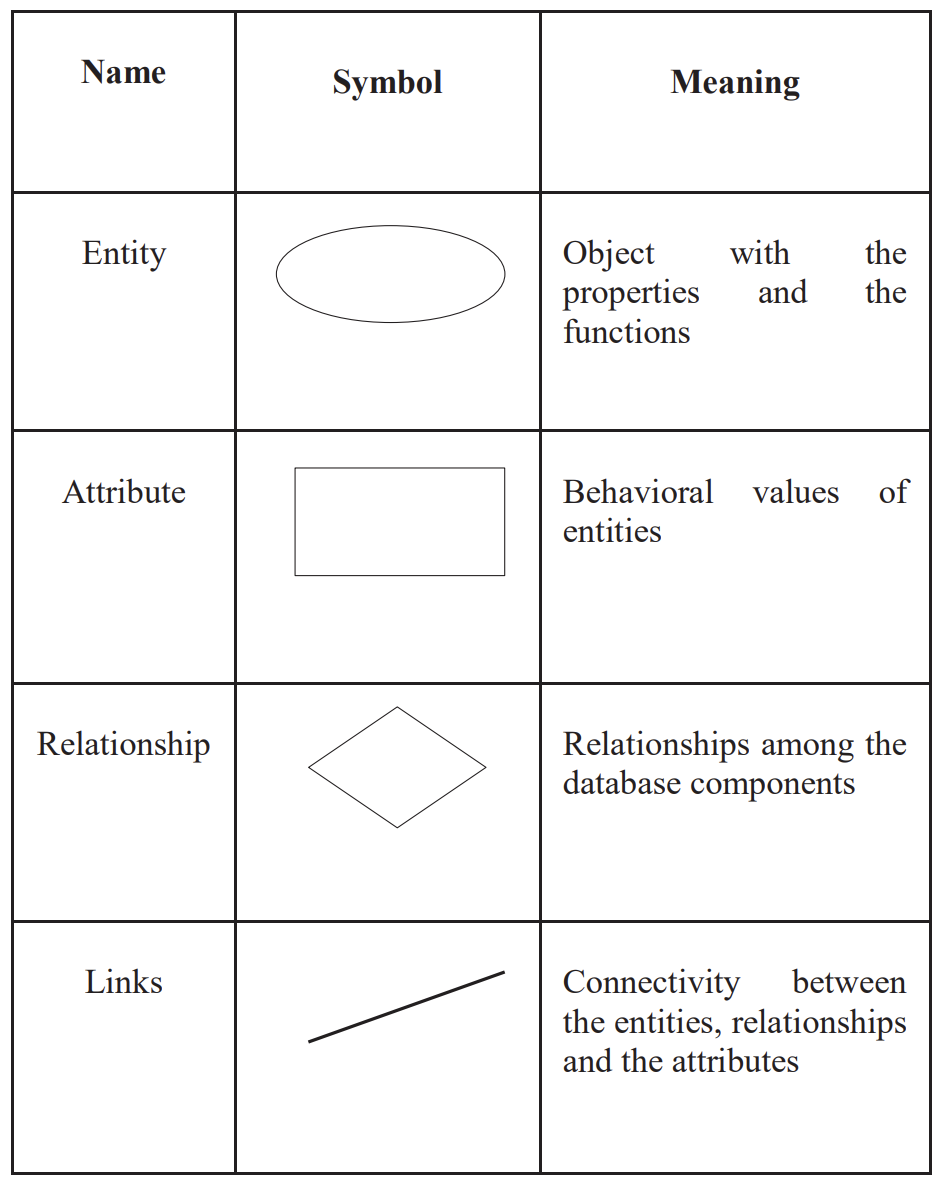
\includegraphics[width=.62\linewidth, center]{images/tinjauan-pustaka/fig-erd.png}
    \caption{Simbol pada ERD (Begum, 2015)}
    \label{fig:erd-notation}
\end{figure}

ERD memiliki tiga komponen utama sebagai notasi. Pertama terdapat entitas, yang merupakan objek yang bersifat konkret maupun abstrak. Pada penerapan di MySQL, objek dapat dituangkan menjadi tabel; Kedua, atribut/field untuk mendeskripsikan karakteristik suatu entitas. Ini akan diimplementasi menjadi kolom dari masing-masing tabel; Terakhir, relasi yang menggambarkan hubungan antar entitas. Misal, Perusahaan memiliki Kapal atau User merupakan bagian dari Perusahaan. Relasi ini kemudian dipetakan bagaimana data berhubungan satu sama lainnya yang terbagi menjadi empat, yaitu:
\begin{enumerate}
    \item One to One (1:1): Setiap entitas A dapat berhubungan paling banyak dengan satu pada himpunan entitas B. Misal, satu Kapal hanya dapat memiliki satu Konfigurasi.
    \item One to Many (1:M): Setiap entitas A dapat berhubungan lebih dari satu anggota entitas B. Misal, satu Perusahaan dapat memiliki banyak Kapal.
    \item Many to One (M:1): Ini merupakan kebalikan dari relasi One to Many. Misal, banyak User dapat mengakses satu Kapal.
    \item Many to Many (M:N): Setiap entity pada kumpulan entitas A dapat berhubungan dengan banyak entitas pada kumpulan entitas B. Misal, banyak User dapat mengakses banyak Kapal.
\end{enumerate}

\section{MySQL}

MySQL adalah sistem manajemen \textit{database open-source} yang umum digunakan sebagai penghubung perangkat lunak dengan \textit{database} server. MySQL dapat secara efektif mengelola banyak pengguna secara bersamaan dan data dalam jumlah masif \parencite{article:gomez}. Kemampuan query yang cukup kuat dan banyaknya dokumentasi menjadi pertimbangan pemilihan database pada sistem yang akan dibangun.

Dalam penelitian ini, MySQL akan digunakan sebagai tempat menyimpan metadata sekaligus data yang dikumpulkan dari sensor. Sistem Monitoring dapat berinteraksi dengan \textit{database} yang dimungkinkan oleh API atau \textit{Application Programming Interface}.


\section{\textit{Application Programming Interface}}
\textit{Application Programming Interface} (API) merupakan sekumpulan aturan dan protocol yang memungkinkan perangkat lunak berbeda untuk berkomunikasi satu dengan lainnya (Raatikainen et al, 2021). Pada pengembangan sistem berbasis web, API dilayani (serve) dalam bentuk tautan atau disebut juga dengan \textit{endpoint} yang memiiki jenis \textit{request} seperti POST, GET, UPDATE, PUT, dan DELETE sehingga klien dapat menyisipkan data atau \textit{payload} ketika melakukan permintaan. Data ini kemudian diolah di server dan diteruskan ke basis data untuk disimpan.

Dalam penelitian ini, tiap \textit{endpoint} akan selalu dilengkapi dengan token autentikasi agar hanya klien yang memiliki otorisasi yang dapat mengirim permintaan ke server. Tiap perangkat IoT yang dipasang akan dilengkapi dengan \textit{authentication key} masing-masing untuk mengidentifikasi sumber perangkat. API digunakan agar memungkinkan perangkat IoT yang dipasang di kapal dapat mengirim data yang diperoleh ke server melalui \textit{endpoint} yang sudah didefinisikan.

\section{Django}

	Django merupakan framework Python dalam pengembangan web. Python adalah bahasa pemrograman populer yang digunakan secara luas di berbagai bidang. Ia terkenal dengan syntaxnya yang singkat dan sederhana, sehingga cocok untuk otomatisasi proses dan pengintegrasian aplikasi \cite{article:buhler}. Popularitas Python dapat dikaitkan dengan kemampuan beradaptasi dan ketersediaan berbagai library dan framework yang mempercepat dan menyederhanakan pengembangan \cite{article:malloy}.

Framework ini akan digunakan untuk menyediakan \textit{Application Programming Interface} (API) agar perangkat IoT dapat mengirim data ke server. Salah satu alasan kuat digunakannya Django adalah menjaga konsistensi tipe data yang dikirim oleh perangkat IoT. Selain itu, adanya library Python seperti Numpy memungkinkan kita untuk mengelola data berukuran masif dengan waktu relatif lebih cepat sehingga ketika pemrosesan data tidak memakan waktu lama.

\section{NextJS}

NextJS merupakan framework Javascript yang menjadi standar dalam pengembangan web modern berbasis JavaScript. JavaScript sendiri merupakan bahasa pemrograman yang sering digunakan khususnya pada pemrograman web. Menurut \textcite{article:tomasdottir}. Umumnya web dengan framework JavaScript dimuat disisi klien atau browser pengguna, disebut juga dengan \textit{Client Side Rendering}  (CSR). Namun, NextJS memungkinkan web untuk dimuat di server terlebih dahulu, disebut juga dengan \textit{Server Side Rendering} (SSR) sehingga web dapat lebih cepat untuk dimuat.

Dalam penelitian ini, NextJS digunakan dalam pengembangan frontend atau tampilan dari sistem. Hal ini digunakan untuk meningkatkan pengalaman pengguna dengan kombinasi fitur CSR dan SSR yang dimiliki NextJS untuk mengelola data serta tampilan dari sistem.

\section{\textit{Whitebox Testing}}

Whitebox testing, dikenal juga sebagai \textit{structural testing} merupakan sebuah metode untuk memeriksa struktur internal dari perangkat lunak menjadi desain test case berdasarkan stuktur kontrol desain (Nidhra and Dondeti., 2012). White box testing merupakan pengujian yang dilakukan untuk menguji perangkat lunak dengan cara mangalisis struktur internal dan kode perangkat lunak. Pengujian ini berfokus pada aliran/flow input dan output dari perangkat lunak. Berikut teknik-teknik struktural pada Whitebox testing:

\begin{enumerate}
    \item Control flow/Coverage testing
    \begin{itemize}
        \item Statement converage
        \item Branch coverage
        \item Decision/condition coverage
        \item Function coverate
    \end{itemize}

    \item Basic path testing
    \begin{itemize}
        \item Flow graph notation
        \item Cyclomatic complexity
        \item Deriving test case
        \item Graph matrices
    \end{itemize}

    \item Loop testing
    \begin{itemize}
        \item Simple loop
        \item Nested loop
        \item Concatenated loop
        \item Unstructured loop
    \end{itemize}

    \item Data flow testing
\end{enumerate}

Pada penelitian ini, pengujian \textit{Whitebox} digunakan untuk memastikan bahwa output dari data yang telah diproses telah sesuai dengan yang diharapkan. Contoh, ketika melakukan konversi log data menjadi nilai \textit{running hour} peneliti harus memastikan penjumlahan data tersebut akan menghasilkan output jam dan menit. Oleh karenanya, pengujian ini sangat penting guna menghasilkan data yang dapat diandalkan ketika diproses di 'Data Processing Layer' sebelum diantar ke 'App Layer'.

\section{\textit{Blackbox Testing}}
\textit{Blackbox testing}, juga dikenal sebagai functional testing merupakan sebuah metode pengujian untuk memverifikasi bahwa sistem telah bekerja dengan semestinya berdasarkan kebutuhan yang telah ditetukan (Noerlina dkk, 2020). Pada metodologi XP, tim pengembang dapat memastikan perangkat lunak telah memenuhi ekspektasi pengguna dan fungsi secara benar tanpa perlu mengetahui bagaimana sistem internal bekerja (Hendri dkk, 2020) yang dimana ini penting untuk memvalidasi behavior perangkat lunak berdasarkan input dan output tanpa menyelidiki kode internal (Ekowati dkk, 2021). Contoh \textit{test case} pada \textit{Blackbox testing} dapat dilihat pada Gambar dibawah.

\begin{figure}[!h]
    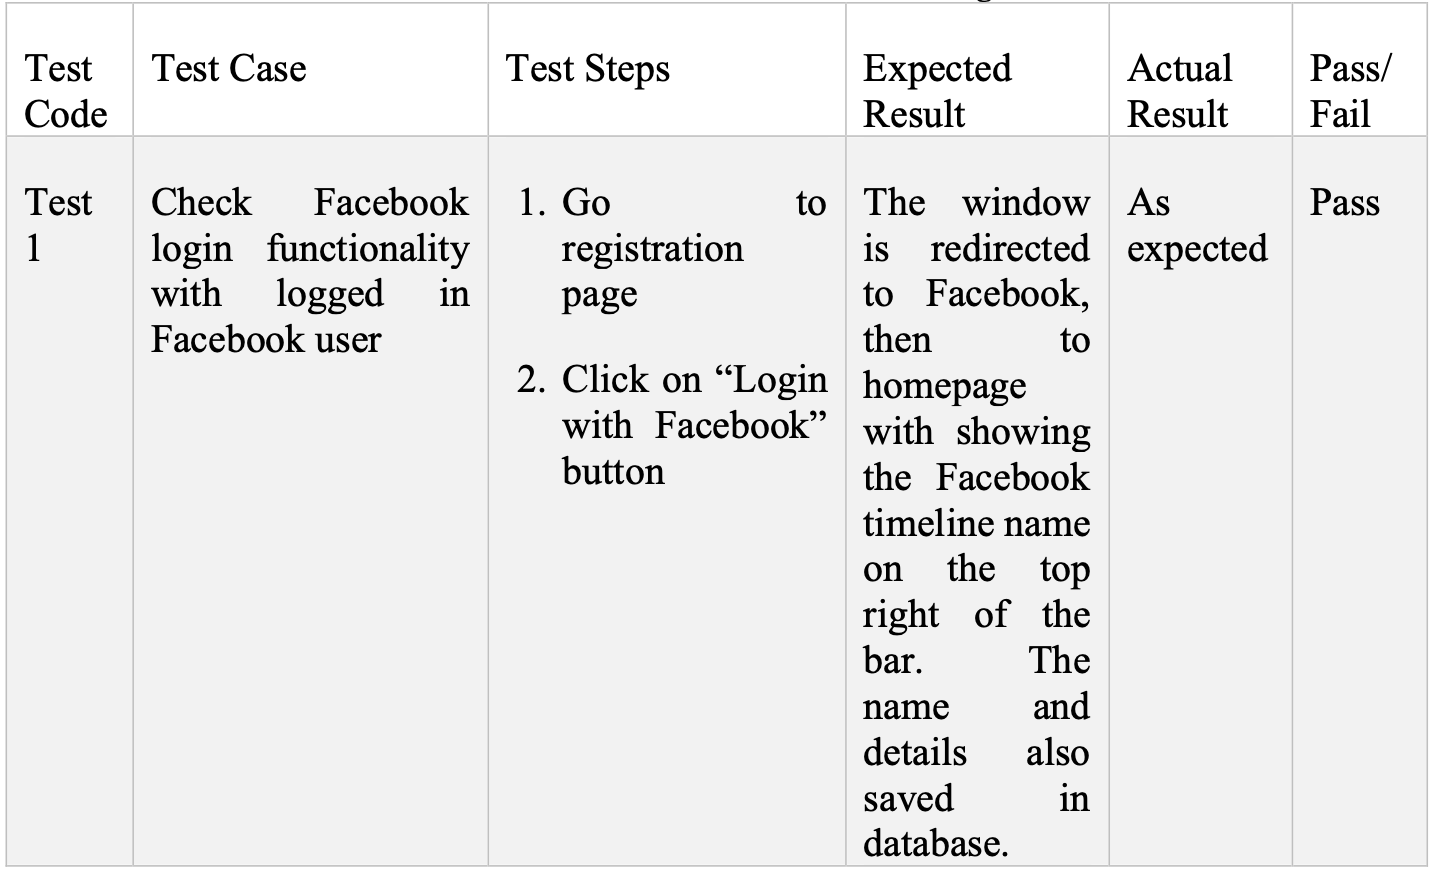
\includegraphics[width=.8\linewidth, center]{images/tinjauan-pustaka/fig-blackbox-eg.png}
    \caption{Contoh Test Case Blackbox Testing (Rahman, 2021)}
    \label{fig:blackbox-example}
\end{figure}

Dalam penelitian ini, \textit{blackbox testing} akan dilakukan setelah kode diunggah ke collective codebase secara bertahap sebagai proses persetujuan mitra. Umpan balik dari mitra akan menentukan apakah task akan dikerjakan sesuai dengan iterasi yang direncanakan atau di iterasi selanjutnya.

\section{Metode Perhitungan Bahan Bakar}

Dokumen Fuel Consumption Rate Verification (FCRV) digunakan sebagai salah satu acuan/bentuk kontrol bahan bakar kapal antara mitra dengan pengguna jasa dan hanya digunakan selama operasi di wilayah pengguna jasa. Dokumen ini berisi informasi kategori operasi berdasarkan rentang kecepatan mesin tertentu. Ini akan digunakan awak kapal ketika hendak melaporkan jumlah konsumsi bahan bakar berdasarkan jumlah running hour pada rentang angka kecepatan yang telah ditentukan. Berikut contoh isi dari Dokumen FCRV.

\newpage

\begin{table}[!h]
    \caption{ Fuel Consumption Rate Verification (PT Bisma Jaya, Fuel Consumption Rate Verification Document. Unpublished confidential document; 2021)}
    \centering
     \begin{tabular}{c c c c}
        \toprule
        Operation Category &
        Max Fuel Used (L) &
        RPM &
        Average Speed (knot) \\ [0.5ex]
        \midrule
        Full Speed          & 28    & 1100      & 5 \\
        Economical Speed    & 18    & 900-1000  & 4 \\
        Slow Speed/Maneuver & 11    & 700-800   & 3 \\
        Idle Speed          & 6     & 600       & 0 \\
        Standby (M/E Off)   & 0     & 0         & 0 \\ [1ex]
        \bottomrule
    \end{tabular}
     \label{tab:fcrv}
\end{table}

Pada tabel diatas, terdapat 4 kategori operasi yakni Full Speed, Economical Speed, Slow Speed/Manuever, dan Idle Speed. Full Speed adalah kondisi kecepatan mesin tertinggi yang hanya digunakan di laut lepas, nilai maksimum konsumsi bahan bakar (FCR) dalam 1 jam mencapai 28L. Lalu, terdapat Economical Speed. Ini merupakan kategori kecepatan tertinggi kedua dan yang paling sering digunakan ketika menyusuri sungai. Kategori ini memiliki rentang RPM 900-1000 dengan nilai FCR 18L dalam 1 jam. Selanjutnya terdapat Slow Speed, dimana kecepatan ini digunakan untuk mengatur posisi kapal di pelabuhan. Kategori ini memiliki rentang RPM 700-800 dengan nilai FCR 11L dalam 1 jam. Terakhir, Idle Speed dimana kapal dalam kondisi tidak bergera namun mesin menyala. Rentang RPM pada kategori ini adalah 700 kebawah dan hanya memakan bahan bakar 6L dalam 1 jam.

Pada praktiknya, awak kapal hanya mengisi nilai running hour dari masing-masing kategori untuk mendapatan nilai konsumsi bahan bakar. Nilai running hour ini sebelumnya didapatkan berdasarkan estimasi mengikuti jurnal aktivitas/pergerakan kapal. Setelah dipasang perangkat IoT di kapal, awak kapal dapat langsung mengikuti nilai running hour berdasarkan tiap kategori yang ditampilkan di sistem. Contoh pengisian tabel pada laporan adalah sebagai berikut.


\begin{table}[!h]
    \caption{Contoh Laporan Penggunaan Bahan Bakar}
    \centering
     \begin{tabular}{c c c}
        \toprule
        Running Hour &
        Operation Category &
        Fuel Consumption (L) \\ [0.5ex]
        \midrule
        01:00   & Full Speed            & 28    \\
        02:30   & Economical Speed      & 45    \\
        00:30   & Slow Speed/Manuever   & 5.5   \\
        00:10   & Idle Speed            & 1     \\
        \textbf{Total}   &              & \textbf{79.5}     \\ [1ex]
        \bottomrule
     \end{tabular}
     \label{tab:fc-report-example}
\end{table}

Metode perhitungan bahan bakar ini nantinya akan diimplementasi pada satu halaman spesifik yang menampilkan konsumsi bahan bakar dalam rentang satu hari. Di halaman ini, pengguna dapat melakukan filter tanggal untuk memudahkan pemantauan data secara historis. Selain pihak manajemen, awak kapal juga dapat mengakses halaman ini sebagai acuan dalam pengisian nilai running hour yang sudah secara otomatis dikategorikan oleh sistem. Halaman ini merupakan salah satu fitur inti dari Sistem Monitoring yang akan dibuat dalam melakukan pemantauan bahan bakar berdasarkan perhitungan yang telah disepakati.

\section{Penelitian Terdahulu}

Berikut rangkuman hasil penelitian terdahulu yang memiliki keterkaitan dengan penelitian yang dilakukan.

\begin{longtable}[!h]
    {
        p{0.05\textwidth}
        p{0.3\textwidth}
        p{0.6\textwidth}
    }
    \caption{Penelitian terdahulu mengenai \textit{Internet of Things} (IoT)}\\

    \hline
        No &
        Nama Peneliti dan Tahun &
        Penelitian yang dilakukan \\ [0.5ex]
    \hline

    \endfirsthead

    % \multicolumn{3}{@{}l}{\ldots continued} \\

    \hline
        No &
        Nama Peneliti dan Tahun &
        Penelitian yang dilakukan \\ [0.5ex]
    \hline
    \endhead % all the lines above this will be repeated on every page
    \hline

    % \multicolumn{3}{r@{}}{continued \ldots} \\
    \endfoot
    \hline
    \endlastfoot

        1
        & \textcite{inproc:abdulmalek}
        &
        \textbf{Judul:}
        \textit{IoT-Based Healthcare-Monitoring System towards Improving Quality of Life: A Review}

        \textbf{Permasalahan:}
        Kelemahan utama dari layanan kesehatan adalah hanya tersedia di rumah sakit, sehingga tidak memadai dan terkadang tidak mampu memenuhi kebutuhan lansia dan penyandang disabilitas. Pemantauan status kesehatan lansia secara real-time adalah masalah yang diselesaikan secara efektif dan praktis oleh \textit{Internet of Things} (IoT) dengan penggunaan data sensor dan telekomunikasi.

        \\

        & &
        \textbf{Hasil:}
        Sistem kesehatan berbasis IoT memfasilitasi hidup orang dalam banyak cara.

        \begin{enumerate}
            \item \textbf{Remote healthcare:}
            Daripada pasien mendatangi layanan kesehatan, solusi nirkabel berbasis IoT menghadirkan layanan kesehatan kepada pasien. Sensor berbasis IoT digunakan untuk mengumpulkan data dengan aman, yang kemudian diproses oleh algoritma kecil dan dibagikan kepada penyedia layanan kesehatan untuk mendapatkan rekomendasi yang tepat.

            \item \textbf{Realtime monitoring:}
            Sensor pemantauan berbasis IoT mengumpulkan serangkaian data psikologis. Penyimpanan data dikelola melalui analisis dan \textit{gateway} berbasis \textit{cloud}.


            \item \textbf{Preventive care:}
            Data sensor digunakan oleh sistem layanan kesehatan IoT untuk memberi tahu anggota keluarga dan membantu deteksi dini keadaan darurat. \textit{Internet of Things} memungkinkan machine learning untuk deteksi anomali dini dan pelacakan tren kesehatan.
        \end{enumerate}

        \\
        \midrule

        2
        & \textcite{article:anh}
        &
        \textbf{Judul:}
        \textit{Development and Implementation of a low-cost IoT System for Small Farm Households}

        \\

        & &
        \textbf{Permasalahan:}
        Pertanian kecil memiliki peran yang yang penting untuk produksi agrikultural terutama pada negara kurang berkembang maupun berkembang. Berbeda dengan pertanian skala besar yang berinvestasi pada teknologi mutakhir untuk memastikan kualitas hasil panen yang maksimal, teknologi pada pertanian kecil masih sangat terbatas.

        \textbf{Hasil:}
        Sistem IoT diusulkan untuk dapat membantu petani kecil meningkatkan kualitas produk pertanian sekaligus mengurangi biaya produksi dan mencegah pemborosan air irigasi dan pupuk. Agrikultur sangat bergantung pada cuaca dan iklim, seperti temperatur dan kadar air tanah. Dalam penelitian, sistem melakukan monitoring pada temperatur, kelembapan, intensitas cahaya, dan kadar air tanah. Parameter tersebut digunakan sebagai acuan dalam mengatur pompa embun, pompa irigasi, jendela ventilasi, kipas ventilasi, dan grow light.

        \\
        \midrule

        3
        & \textcite{inproc:hizbullah}
        &
        \textbf{Judul:} \textit{Internet of Things} for Smart Transportation in North Moluccas Province

        \textbf{Permasalahan:} Perlunya transportasi yang lebih aman dan penyediaan layanan keselamatan selama keadaan darurat di wilayah Provinsi Maluku Utara.

        \\

        & &
        \textbf{Hasil:} Diterapkan otomasi pada sistem navigasi yang dapat membantu meningkatkan akurasi dan keandalan navigasi perahu agar mengurangi risiko kecelakaan. Peneliti juga menerapkan sistem monitoring yang dapat menyediakan data secara real-time terhadap kondisi perahu untuk kebutuhan maintenance dan deteksi lebih awal isu yang mungkin akan terjadi.

        \\
        \midrule

        4
        & \textcite{article:maswadi}
        &
        \textbf{Judul:} \textit{Systematic Literature Review of Smart Home Monitoring Technologies Based on IoT for the Elderly}

        \textbf{Permasalahan:} Dengan seiring bertambahnya populasi lansia berumur 65 keatas di negara-negara seperti Amerika, Jerman, Perancis, Itali, dan Jepang terdapat kemungkinan mereka akan beban yang bertambah pada kesehatan dan layanan sosial. Diperlukan teknologi yang dapat memberikan lingkungan hidup yang kondusif bagi para lansia.

        \textbf{Hasil:} Penerapan teknologi sistem smart home pada lansia telah secara signifikan meningkatkan kualitas hidup diantara para lansia. Beberapa teknologi yang dilaporkan telah menyelamatkan hidup para lansia di situasi darurat.

        \\
        \midrule

        5
        & \textcite{article:song}
        &
        \textbf{Judul:} \textit{Internet of Maritime Things Platform for Remote Marine Water Quality Monitoring}

        \textbf{Permasalahan:} Penerapan sistem monitoring kualitas air di laut memerlukan dukungan komunikasi jarak jauh dan berkecepatan tinggi yang stabil.

        \textbf{Hasil:} Dalam penelitian ini, dikembangkan sebuah platform IoT Maritim yang mendukung komunikasi jarak jauh dan berkecepatan tinggi untuk pemantauan kualitas air laut jarak jauh dan online. Perangkat ditempatkan di atas permukaan air laut dan gerbang untuk pengiriman data ditempatkan darat. Untuk merealisasi komunikasi jarak jauh dan berkecapatan tinggi antara perangkat dengan control center di darat, dikembangkan sistem penyesuaian sinar otomatis (automatic beam adjustment system) untuk antena pengarah sehingga dapat mendukung komunikasi jarak jauh dan berkecepatan tinggi dengan secara otomatis mengatur derajat sinar agar selalu mengarah ke gateway di darat. Metode ini terbukti memberikan performa komunikasi dua kali lipat dibandingkan koneksi nirkabel (LTE di laut) yang ada.

        \\

    \label{tab:prev-papers}
\end{longtable}